
在开始学习线程安全的数据结构之前,我们必须知道它们是什么。如果这看起来像是一个简单的问题——多个线程可以同时使用的数据结构——那么你对这个问题的认识还远远不够。当开始设计并发程序中使用的新数据结构或算法时,就知道这个问题是多么的重要了,以至于怎么强调都不为过。如果这句话让你感到警惕,并停下来思考,那最好了。我刚刚暗示线程安全的数据结构没有一个明确定义适合每种需求和应用程序,事实也如此。

\subsubsubsection{7.2.1\hspace{0.2cm}线程安全的最佳方式}

让我们从一些简单的,但在实践中经常遗忘的开始:高性能设计的一个原则是,不做事总是比做事快。当前,这个原则可以缩小为:对于数据结构,是否需要线程安全?确保线程安全,意味着需要由计算机完成一些工作。问问自己,真的需要它吗?是否可以对计算进行调度,使每个线程都有自己的数据集进行操作?

一个例子是我们在前一章中使用的线程安全计数器。如果需要所有线程始终看到计数器的当前值,那么这就是正确的解决方案。但当所需要的只是计算在多个线程上发生的事件,例如:在分配给多个线程的一组大数据中搜索某些内容。线程在执行搜索时不需要知道计数的当前值。当然,需要知道计数的最新值来增加它,这是正确的,只有在所有线程上增加单个共享计数时,才会出问题,就像这样:

\hspace*{\fill} \\ %插入空行
\noindent
\textbf{01a\_shared\_count.C}
\begin{lstlisting}[style=styleCXX]
std::atomic<unsigned long> count;
…
for ( … counting loop … ) { // On each thread
	… search …
	if (… found …)
	count.fetch_add(1, std::memory_order_relaxed));
}
\end{lstlisting}

计数的性能非常差,可以看到在基准测试中,我们只做计数(不搜索):

%\hspace*{\fill} \\ %插入空行
\begin{center}
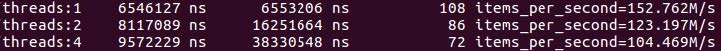
\includegraphics[width=0.9\textwidth]{content/2/chapter7/images/1.jpg}\\
图7.1 - 如果计数是共享的,那么对多个线程的计数不会改变
\end{center}

计数的改变实际上是负的:在两个线程上获得相同的计数值要比在一个线程上花费更长的时间(尽管我们尽了最大努力使用无等待的计数,同时使用最快的内存序)。当然,如果搜索比计数要长,那么计数的性能就无关紧要了(但搜索代码本身也可以在全局数据上做一些事,或者在每个线程的副本上做一些事,所以这是一个有指导意义的例子)。

假设我们只关心计算结束时的计数值,一个更好的解决方案是,在每个线程上保持本地计数,并且只增加共享计数一次:

\hspace*{\fill} \\ %插入空行
\noindent
\textbf{01b\_per\_thread\_count.C}
\begin{lstlisting}[style=styleCXX]
unsigned long count;
std::mutex M; // Guards count
…
// On each thread
unsigned long local_count = 0;
for ( … counting loop … ) {
	… search …
	if (… found …) ++local_count;
}
std::lock_guard<std::mutex> L(M);
count += local_count;
\end{lstlisting}

为了强调共享计数增量现在不重要的,我们将使用互斥锁对其进行保护。通常,锁是更安全的选择,因为它更容易理解(因此,更难制造Bug),尽管在计数的情况下,原子整数实际上会让代码更简单。

如果每个线程在到达结束之前多次增加本地计数,并且必须对共享计数进行增加的操作,那么这种改变几乎完美:

%\hspace*{\fill} \\ %插入空行
\begin{center}
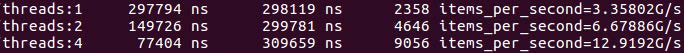
\includegraphics[width=0.9\textwidth]{content/2/chapter7/images/2.jpg}\\
图7.2 - 计数在多个线程上完美地与每个线程的计数
\end{center}

因此,最好的线程安全是,即不需要多个线程访问共享数据。通常,这种安排会以一些开销为代价的,例如:每个线程维护一个容器或内存分配器,其大小会不断地改变。如果在程序结束之前不将内存释放给主分配程序,就可以避免锁定。代价是一个线程上未使用的内存不能提供给其他线程使用,因此总的内存使用将是所有线程的峰值使用的总和,即使这些峰值使用时刻发生在不同的时间。这是否可以接受取决于问题的细节和实现:这是每个开发者都必须考虑的问题。

当涉及到线程安全时,可以说这个方案选择了逃避。从某种角度来看,确实如此,但在实践中经常出现这样的情况:在不需要共享数据结构的地方使用共享数据结构,并且性能提高非常显著,因此需要强调这一点。现在是时候来看看真正的线程安全了,其中数据结构必须在线程之间共享。

\subsubsubsection{7.2.2\hspace{0.2cm}真正的线程安全}

假设我们确实需要同时从多个线程访问特定的数据结构,现在就必须讨论线程安全了。但现在还是没有足够的信息来确定线程安全意味着什么。我们已经在前一章中讨论了强线程和弱线程安全保证。本章中,即使这样分区也不够,所以我们不应该讨论一般的线程安全,而是应该描述数据结构提供并发访问的保证。

正如我们所看到的,弱(但通常很容易提供)保证只要数据结构保持不变,多个线程就可以读取相同的数据结构。显然,最有力的保证是,任意数量线程可以随时执行任何操作,并且数据结构保持在良好定义的状态。这种保证通常既昂贵又不必要。程序可能需要数据结构支持的某些(但不是所有)操作提供这样的保证。还有其他的简化版本,比如:限制访问数据结构的线程数量。

作为一个规则,想要提供尽可能少的保证来保证程序是正确的,而不是更多:线程安全特性通常非常昂贵,甚至不使用时也会产生开销。

考虑到这一点,让我们开始研究具体的数据结构,并看看如何提供不同级别的线程安全。

































